There are jobs that are trivial to all people but they are extremely difficult even for the most powerful and sophisticated software and machines. This type of task has as its characteristics the need for creativity, emotional sensibility, empathy, sarcasm and level of abstraction which, in the present moment, is inherited in the minds of human beings.

There are still cases where automatic methods can accomplish the task, but the necessary resources do not exist as examples of bases or a well-defined set of rules.
Some examples classify this type of task as image recognition, especially when there is occlusion or involves subjective analysis, content authorship, analysis of emotions and so many other activities that inherently require human intelligence to be performed. Luis von Ahn introduced in his dissertation  \cite{VonAhn:2005:HC:1168246}  a paradigm named Human Computation that allows approaching the problems from this point of view, identifying in it what tasks can be automated and which ones require human treatment. Additionally, Human Computation can improve performance by the division of labor because it helps to define tasks that can be executed in parallel  \cite{Rohwer:2010:NHC:1837885.1837897}.

One of the benefits of modeling a system according to the Human Computation paradigm is to focus the effort of human collaborators only on tasks that really require their attention, this is done by identifying the tasks that inherently require human intelligence. Each of these tasks is a HIT (Human Intelligence Task) and corresponds to something that humans can easily solve while a machine presents extreme difficulty in trying to solve \cite{doi:10.2200/S00371ED1V01Y201107AIM013}. 

In short, Human Computation is a paradigm that proposes to identify in a problem which tasks require human intelligence and which tasks can be automated. In general, the problems that might benefit by using Human Computation modeling are problems in which it is possible to identify tasks that are very difficult for machines but can be easily completed by humans. This strategy is illustrated in Figure~\ref{hc}.

\begin{figure}[ht]
\centering
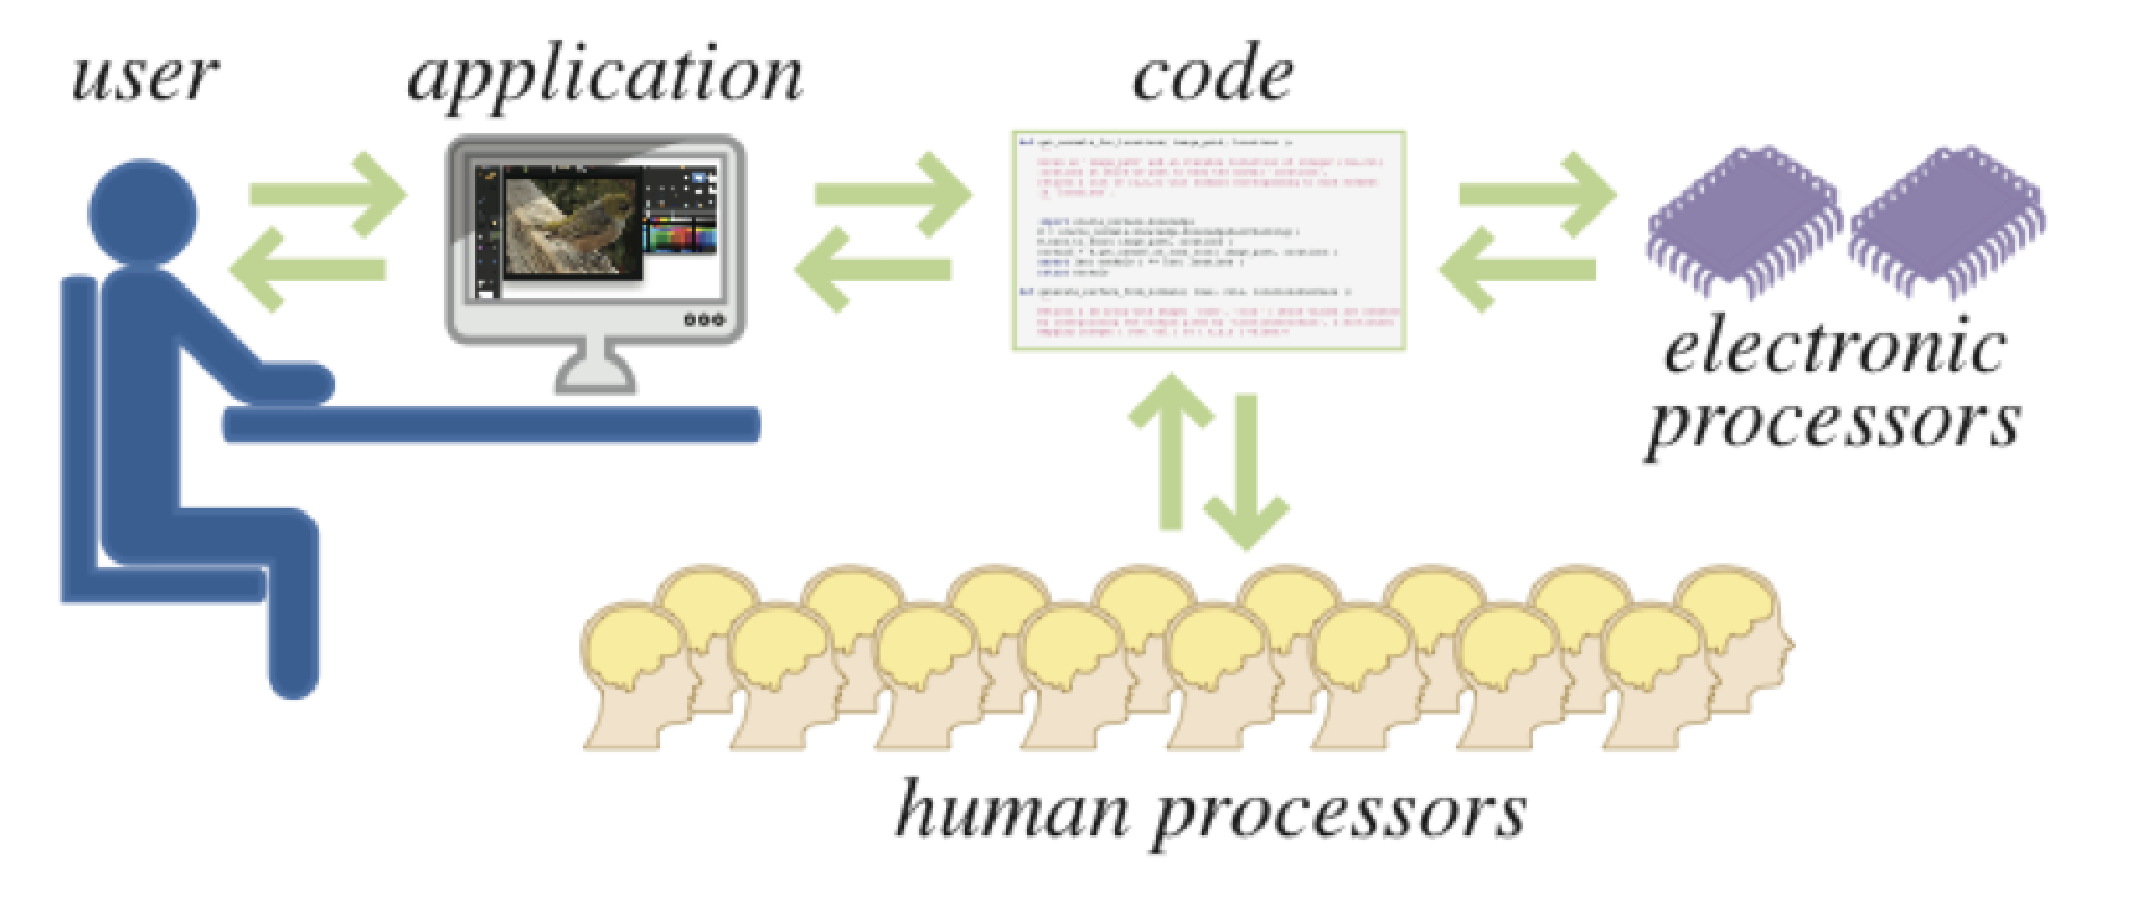
\includegraphics[scale=0.19]{figure/hc}
\caption{General human computation architecture}
\label{hc}
\end{figure}

A HIT may involve creative activities such as authorship, simple observation as in identifying events in videos, or empathy such as the detection of emotion in facial expression images, but all these tasks can still be performed by people more easily than it would be for the machines. In terms of complexity, a HIT can range from a trivial microtask to a complex macrotask.

Macrotasks require more effort from the worker, often requiring him to be an expert in the field or to have training on subjects related to the task. In the context of media annotation, this kind of task is suitable for complex annotations because it assumes that the worker is qualified and will devote the time and effort required to complete it. However, macrotasks often require sophisticated annotation systems and limit the group of workers who are able to execute them \citep{Haas:2015:AMC:2824032.2824062}. In this work, complex annotations are defined as those that combine annotations on different aspects of annotated objects and therefore are usually obtained by macrotasks.

On the other hand, microtasks are usually modeled in a way that can be accomplished quickly and easily by less skilled workers. For media annotation, this kind of task is usually used to generate simple annotations, which refer to one or a few items to be annotated in each task. Often a Microtask can be performed using a simple annotation tool. Microtasks are widely used in crowdsourcing projects and this kind of task is supported by well-established commercial platforms such as Amazon Mechanical Turk, CrowdFlower, and Microworkers. According this approach microtasks should be:
\begin{itemize}
	\item{\textbf{Small:}} a worker must complete a task by means of few interactions, preferably by a single interaction.
	
	\item{\textbf{Quick:}} it should be possible to complete a task in a very short time, preferably within a few minutes.

	\item{\textbf{Easy:}} the easier the task, the less skilled the workers should be. Preferably, a task must be modeled so that it can be performed by any worker, just read the instructions and have the technical requirements for the task, such as minimal screen resolution, audio devices, or Internet connection speed.
\end{itemize}

Moreover, considering each microtask as a human computation function, mapping elements from input to output, it is possible to compose an algorithm using these functions to obtain equivalent results generated by macrotasks \cite{Chen:2017:RIM:3025453.3025969}.


